\documentclass[e2_tp1_main.tex]{subfiles}

\begin{document}

\section{Introducci\'on}

En el presente informe, se dise\~nar\'a una fuente regulada de tensi\'on, realizando un an\'alisis te\'orico de su funcionamiento, simulando el mismo en LtSpice y finalmente verificando que esto se cumpla con mediciones en el circuito real. 

Los requerimientos para el dise\~no son:
\begin{table}[ht!]
	\centering
	
	\begin{tabular}{|c|c|}
		\hline 
		$V_{O}$ [V] & $I_{O\, MAX}$ [A] \\ 
		\hline \hline
		9 $< V_O <$ 15 & 1.5 \\ 
		\hline 
		\end{tabular} 	
	
	\caption{Requerimientos de la fuente regulada de tensi\'on a dise\~nar.}
	\label{table:reqs}
\end{table}

Como la tensi\'on de salida no necesita llegar a 0V en regulaci\'on, se decidi\'o utilizar la configuraci\'on no inversora vista en clase (donde la tensi\'on de salida siempre es mayor a la de referencia).

\begin{figure}[htb]
	\centering
	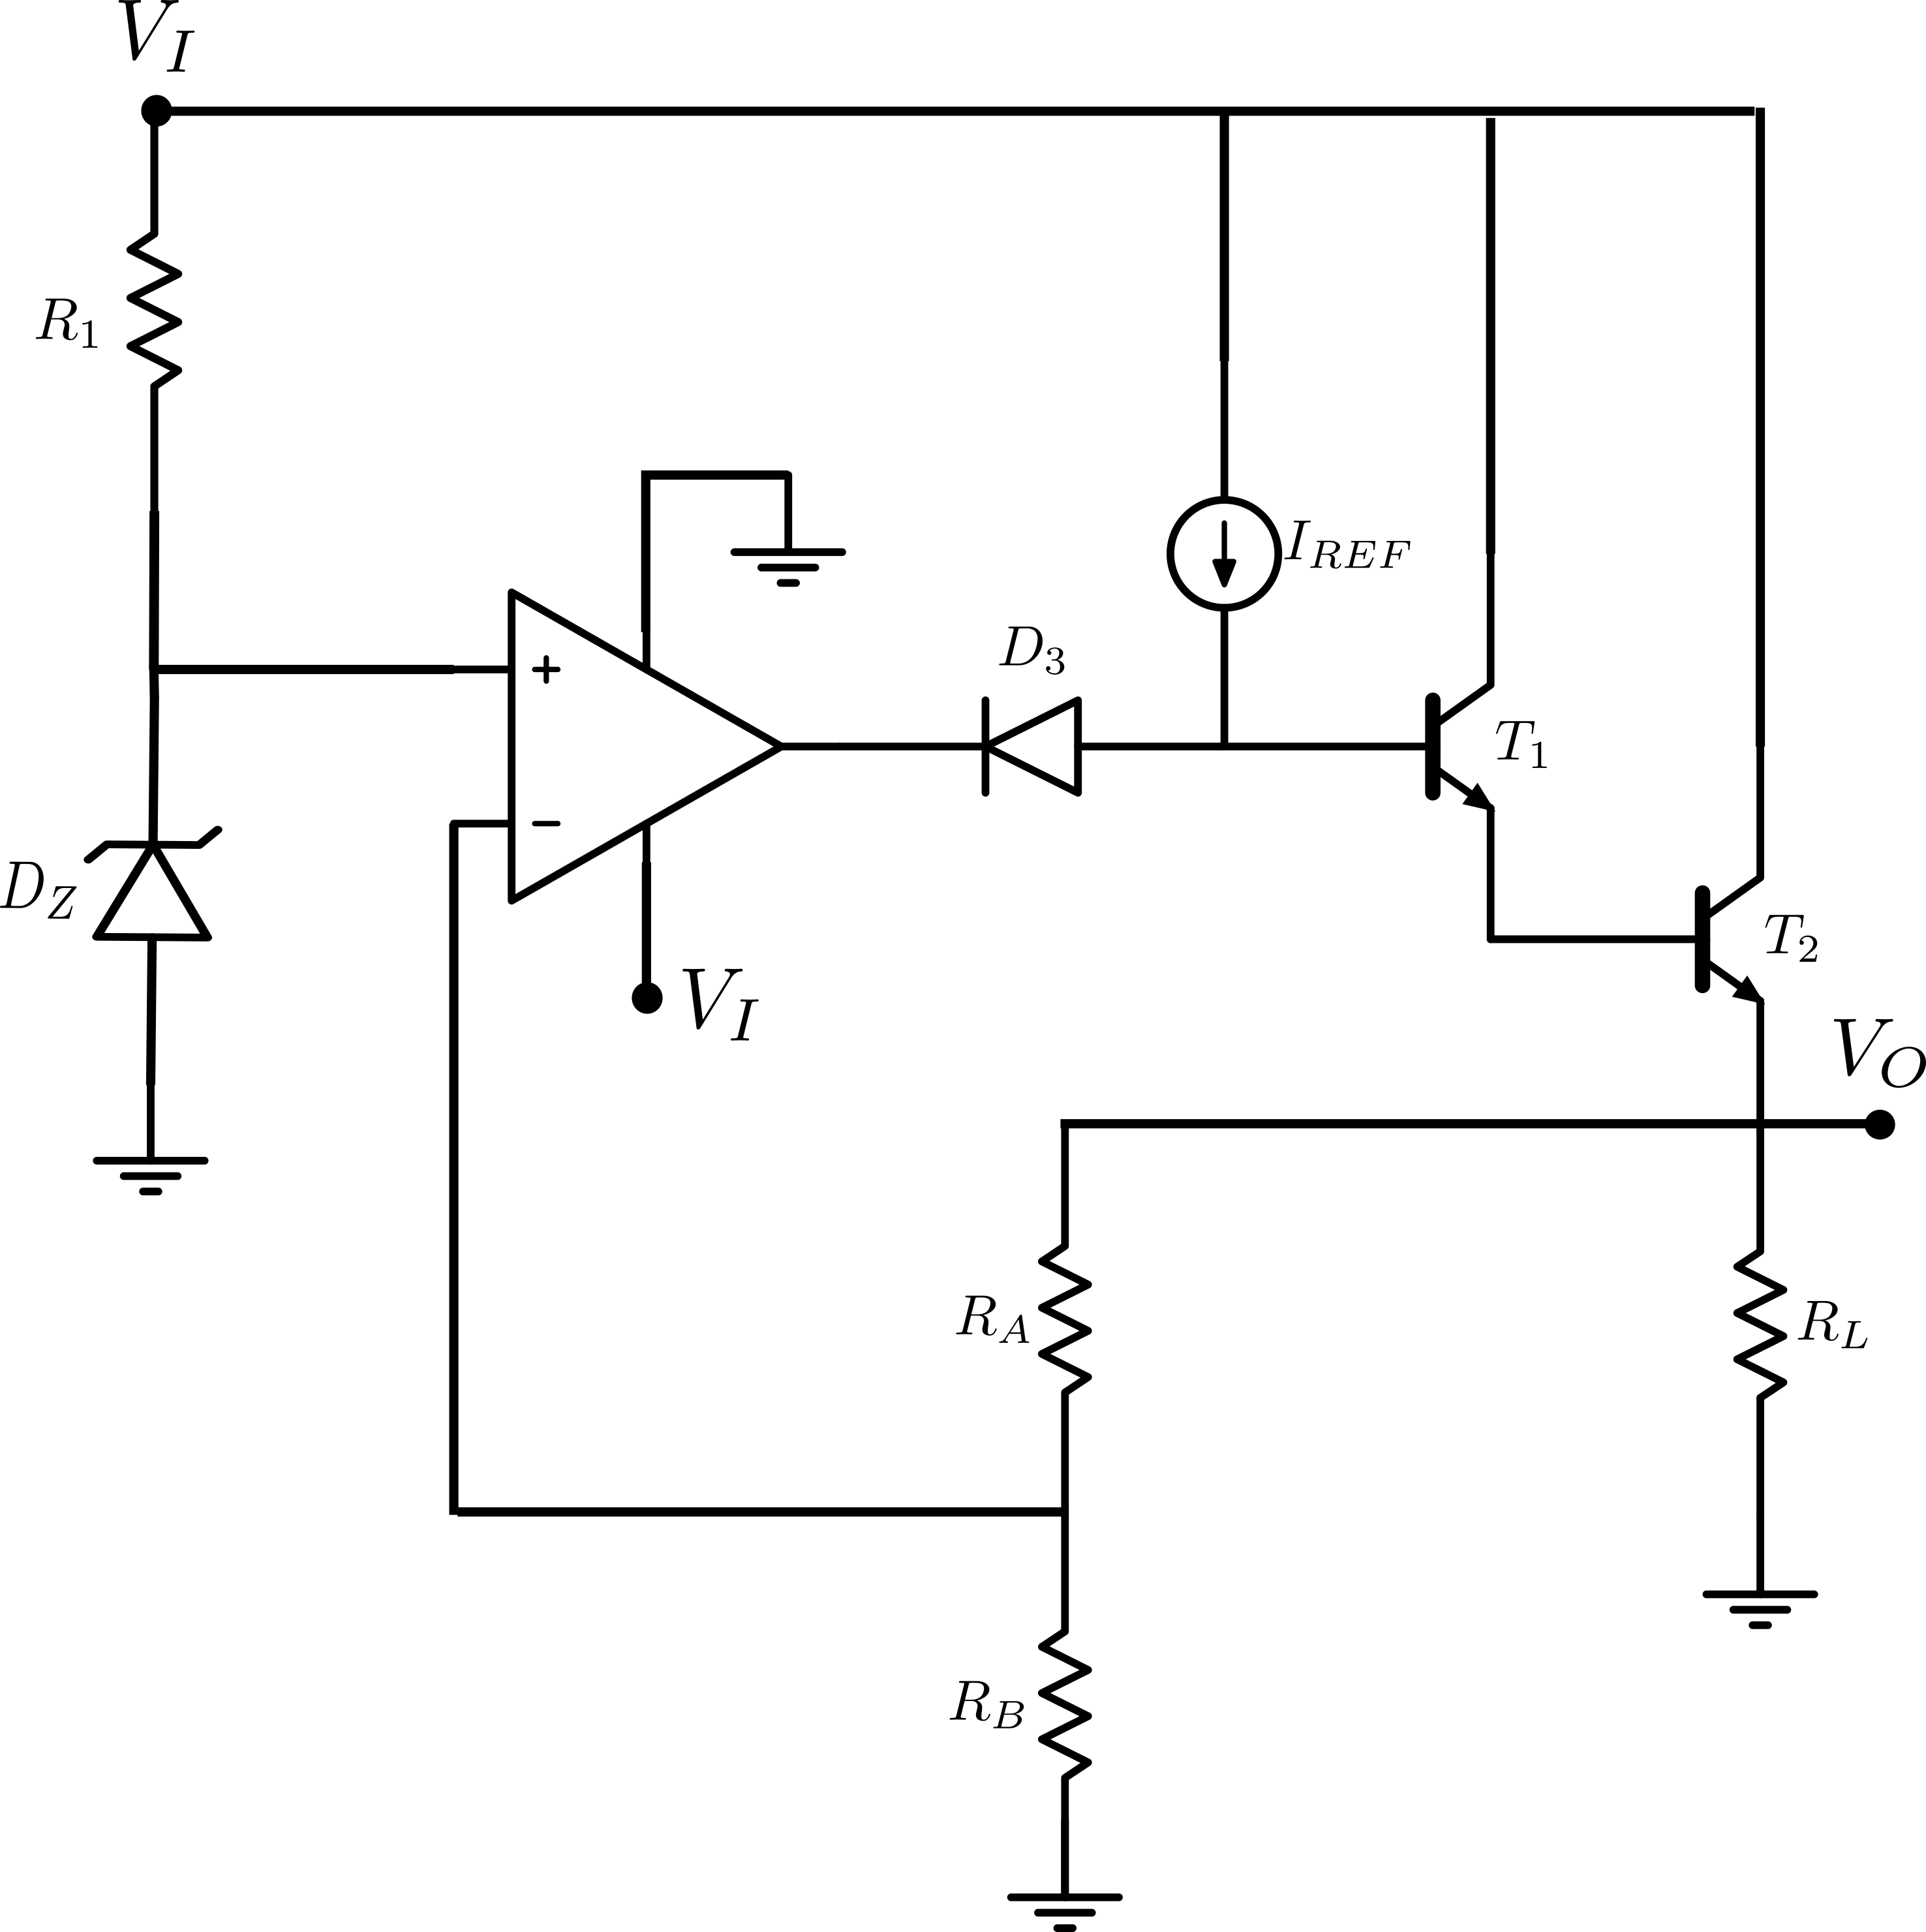
\includegraphics[width=0.8\textwidth]
	{circuitos/circuito.png}
	\caption{Dise\~no b\'asico de la fuente regulada de tensi\'on}
	\label{fig:circ3}
\end{figure}

\section{Dise\~no de la fuente regulada de tensi\'on}

El circuito b\'asico del que se parti\'o (como se observa en la figura \ref{fig:circ3}) obtiene la tensi\'on de referencia a partir de un diodo Zener, que es comparada mediante un opamp con un divisor resistivo de la tensi\'on de salida. Despreciando la corriente que entra al operacional, la salida se obtiene como:

\begin{equation}
	V_{O} = \left( 1+\frac{R_A}{R_B} \right) \cdot V_Z
\end{equation}

De esta manera, cambiando el valor de $R_A$ se puede variar la tensi\'on de salida. 

La realimentaci\'on se completa con el par Darlington y la fuente de corriente. El par funciona como transistor de paso, aportando la diferencia de tensi\'on necesaria para que $V_{O}$ sea la de regulaci\'on. La realimentaci\'on del circuito hace que el opamp consuma la corriente suficiente como para que a la base de $T_1$ llegue la justa y necesaria para que la salida se mantenga en regulaci\'on. El diodo $D_1$ impide que el opamp entregue corriente, con lo cual la corriente m\'axima de salida se tiene cuando la totalidad de la entregada por la fuente va al transistor.

\subsection{Generador y detector}

Para obtener el rango establecido en la tabla \ref{table:reqs}, se decidi\'o utilizar un diodo Zener con tensi\'on nominal de 8.2V, de forma tal que con $R_B=47\mathrm{k}\Omega$ y utilizando un preset de 50k$\Omega$ como $R_A$, se puede llegar a los valores de $V_O$ requeridos. Si bien el valor exacto de los componentes no es particularmente relevante en el circuito, se eligieron en este orden de magnitud con el objetivo de que circule por ellos una corriente relativamente peque\~na (de alrededor de $\nicefrac{V_Z}{R_B}\simeq 0.17\mathrm{mA}$), sin introducir el ruido que una resistencia del orden de los megaohms provocar\'ia.

En cuanto a $R_1$, la presencia de la misma tiene el \'unico prop\'osito de llevar al Zener a regulaci\'on. De acuerdo a la hoja de datos de este componente\footnote{
\url{https://www.onsemi.com/pub/Collateral/1N5221B-D.PDF}, consultada 18/04/19. 
}, para que esto ocurra, la corriente debe ser mayor a $I_{ZK}=0.5$mA, con valor nominal de $I_{ZT}=20$mA, con su l\'imite superior dado por la potencia de 0.5W que se puede disipar (si bien se trabaj\'o \'ordenes de magnitud por debajo de este l\'imite, para que el diodo no caliente). En nuestro circuito, esta corriente est\'a dada por:
\[I_Z= \frac{V_{I} - V_{Z}}{R_1} \]

Por lo tanto, sus m\'inimos y m\'aximos coincidir\'an con los de la tensi\'on de entrada. Se consider\'o que la tensi\'on m\'inima de entrada es $V_{I\, MIN} = V_{O\, MIN} + 1.5\mathrm{V} = 10.5\mathrm{V}$, y la m\'axima,  $V_{I\, MAX} = V_{O\, MAX} + 5\mathrm{V} = 20\mathrm{V}$ (sobredimensionando en ambos casos). Se eligi\'o entonces $R_1=560\Omega$, con lo cual se obtiene $I_{Z\, MIN} = 4.1$mA e $I_{Z\, MAX} = 21.1$mA.


\subsection{Circuito de control: par Darlington}

Se decidi\'o utilizar dos transistores para el Darlington, en lugar de un integrado, para tener m\'as control sobre el dise\~no del mismo. Por ejemplo, la mayor\'ia de los pares Darlington del pa\~nol de la universidad poseen resistencias entre la base y el emisor de $T_2$, y lo mismo para $T_1$. Sin embargo, con los transistores elegidos (como se ver\'a a continuaci\'on), estas resistencias no ayudan a llevar los $\beta$ a un punto mejor, y por lo tanto se decidi\'o obviarlas.
 
A la hora de elegir $T_1$ y $T_2$, la principal consideraci\'on que se tuvo es que pudieran soportar holgadamente la corriente m\'axima. En segundo lugar, se tuvo en cuenta los rangos de $\beta$ aportados por el fabricante, buscando el mayor m\'inimo y la menor dispersi\'on posible. Por \'ultimo, se consider\'o tambi\'en el precio de cada componente listado en el pa\~nol de la universidad.


\subsubsection{Elecci\'on de $T_2$}

Para $T_2$, sabemos que debe soportar toda la corriente de salida. Como debemos asegurar que se llegue por lo menos a 1.5A, y este valor depender\'a considerablemente de los $\beta$, se descargaron modelos que s\'olo garantizacen correcto funcionamiento hasta 2A o menos. Dejando de lado tambi\'en los que est\'an dise\~nados para m\'as de 15A (los cuales suben mucho de precio y pierden demasiado $\beta$, y sabemos que no trabajaremos con corrientes tan elevadas), quedaron los modelos listados en la tabla \ref{table:modelos-t2}.

\begin{table}[ht!]
	\centering
	\begin{tabular}{|c|c|c|c|c|}
		\hline 
		Modelo & $I_{C\, MAX}$ (A) & $\beta_{MIN}$ (veces) & $\beta_{MAX}$ (veces) & Precio (USD) \\ 
		\hline \hline
		TIP31C & 3 & 10 & 50 & 0.26 \\ 
		\hline 
		TIP41A & 6 & 15 & 75 & 0.28 \\ 
		\hline 
		TIP3055 & 15 & 20 & 70 & 0.43 \\ 
		\hline 
		\end{tabular} 	
	\caption{Caracter\'isticas de los modelos considerados para $T_2$}
	\label{table:modelos-t2}
\end{table}

Se observa en dicha tabla el TIP41A posee un $\beta$ un 50\% mayor y el doble de corriente, por s\'olo dos centavos de d\'olar m\'as. Si bien en este circuito 3A son suficientes, puesto que el TIP41A est\'a dise\~nado para trabajar con corrientes muy superiores a las que necesitamos, mantiene para $I_{O} = 2$A su valor de $\beta$ casi sin ca\'ida, lo cual no ocurre con el TIP31C. En cuanto al TIP3055, la corriente que soporta es innecesariamente alta, y el $\beta$ es de similares caracter\'isticas al del TIP41A. Como su precio es considerablemente superior al de los otros transistores sin mejoras considerables respecto del TIP41A, se descart\'o. Se utiliz\'o pues el 41A. Por lo discutido en cuanto a las caracter\'isticas de su $\beta$ en las corrientes que utilizaremos, se decidi\'o no agregar resistencias al par Darlington.


\subsubsection{Elecci\'on de $T_1$}

Si sobredimensionamos la corriente m\'axima de salida un 10\% (puesto que debemos asegurar que se llegue a 1.5A, y por lo tanto dise\~nar para llegar a m\'as), el otro transistor debe soportar una corriente m\'axima de:

\[I_{T_1\, MAX} = 
\frac{I_{T_2\, MAX}}{\beta_{T_2\,MIN}} \leq
\frac{1.65\mathrm{A}}{15} = 110\mathrm{mA} \]

N\'otese que incluso considerando 2A se obtienen valores inferiores a 200mA, y s\'olo con 1.5A se obtiene 100mA, con lo cual podemos decir con confianza que $I_{T_1\, MAX}$ debe ser superior a 100mA. Descartando los que soportan m\'as de 1A, quedan s\'olo el 2N3904 y el BC337. Si bien este \'ultimo cuesta un poco m\'as del doble (0.10U\$D contra 0.04U\$D), se eligi\'o este modelo de todas maneras por los siguientes motivos:

\begin{itemize}
	\item Ambos tienen el mismo $\beta$ m\'inimo, pero el m\'aximo del BC337 es el doble de grande.
	\item Con $I_C = 100$mA, el $\beta$ del 2N3904 se reduce un 70\%, mientras que la curva del BC337 se encuentra en su m\'aximo en este punto.
	\item El BC est\'a dise\~nado espec\'ificamente para amplificaci\'on, y el 2N es de uso general.
\end{itemize}

  
 \subsection{Amplificador de error}

En esta fuente regulada, el amplificador de error consiste en un opamp, que compara (resta) la tensi\'on de referencia, generada por el Zener, con una fracci\'on de la de salida. A la salida del operacional se tendr\'a la tensi\'on necesaria para minimizar el error. 

Este operacional debe contar con la posibilidad de ser alimentado con $0 - V_{CC}$, en lugar de $\pm V_{CC}$, puesto que se lo alimentar\'a con la tensi\'on de entrada. Debido a limitaciones en la disponibilidad de componentes en el pa\~nol, la \'unica opci\'on disponible que cumpl\'ia con nuestros requisitos fue el LM358. Sin embargo, esto no implica que no sea adecuado para la aplicaci\'on que le daremos: con 100dB de PSRR, y 100dB tambi\'en de ganancia, se adapta perfectamente al uso que le daremos, en el cual la alimentaci\'on no ser\'a necesariamente estable (pues es la entrada) y se requiere la mayor ganancia posible. A su vez, el fabricante asegura que este integrado puede sinkear m\'as de 10mA, con lo cual ser\'a capaz de aceptar toda la corriente de referencia sin quemarse.


\subsection{Pre-regulador: fuente de corriente}

La fuente de corriente que se utiliz\'o se observa en la figura \ref{fig:fuente}. El funcionamiento de la misma es el siguiente: la resistencia $R_5$ permite que se polaricen los diodos en directa, generando en la base de $T_3$ una tensi\'on de $V_{B_3}=V_{I} - 2 V_D \simeq V_{in} - 1.4\mathrm{V}$. Luego, cuando el transistor est\'e correctamente polarizado (lo cual depender\'a de la diferencia entre $V_I$ y $V_O$), en la resistencia $R_6$ caer\'a una tensi\'on de $V_{R_6} = V_I - V_{E_3} = V_I - (V_{B_3} + V_{BE_3}) = V_I - (V_I - 2V_D + V_{BE_3}) = V_D$ si consideramos $V_{BE_3} = V_D$.

\begin{figure}[htb!]
	\centering
	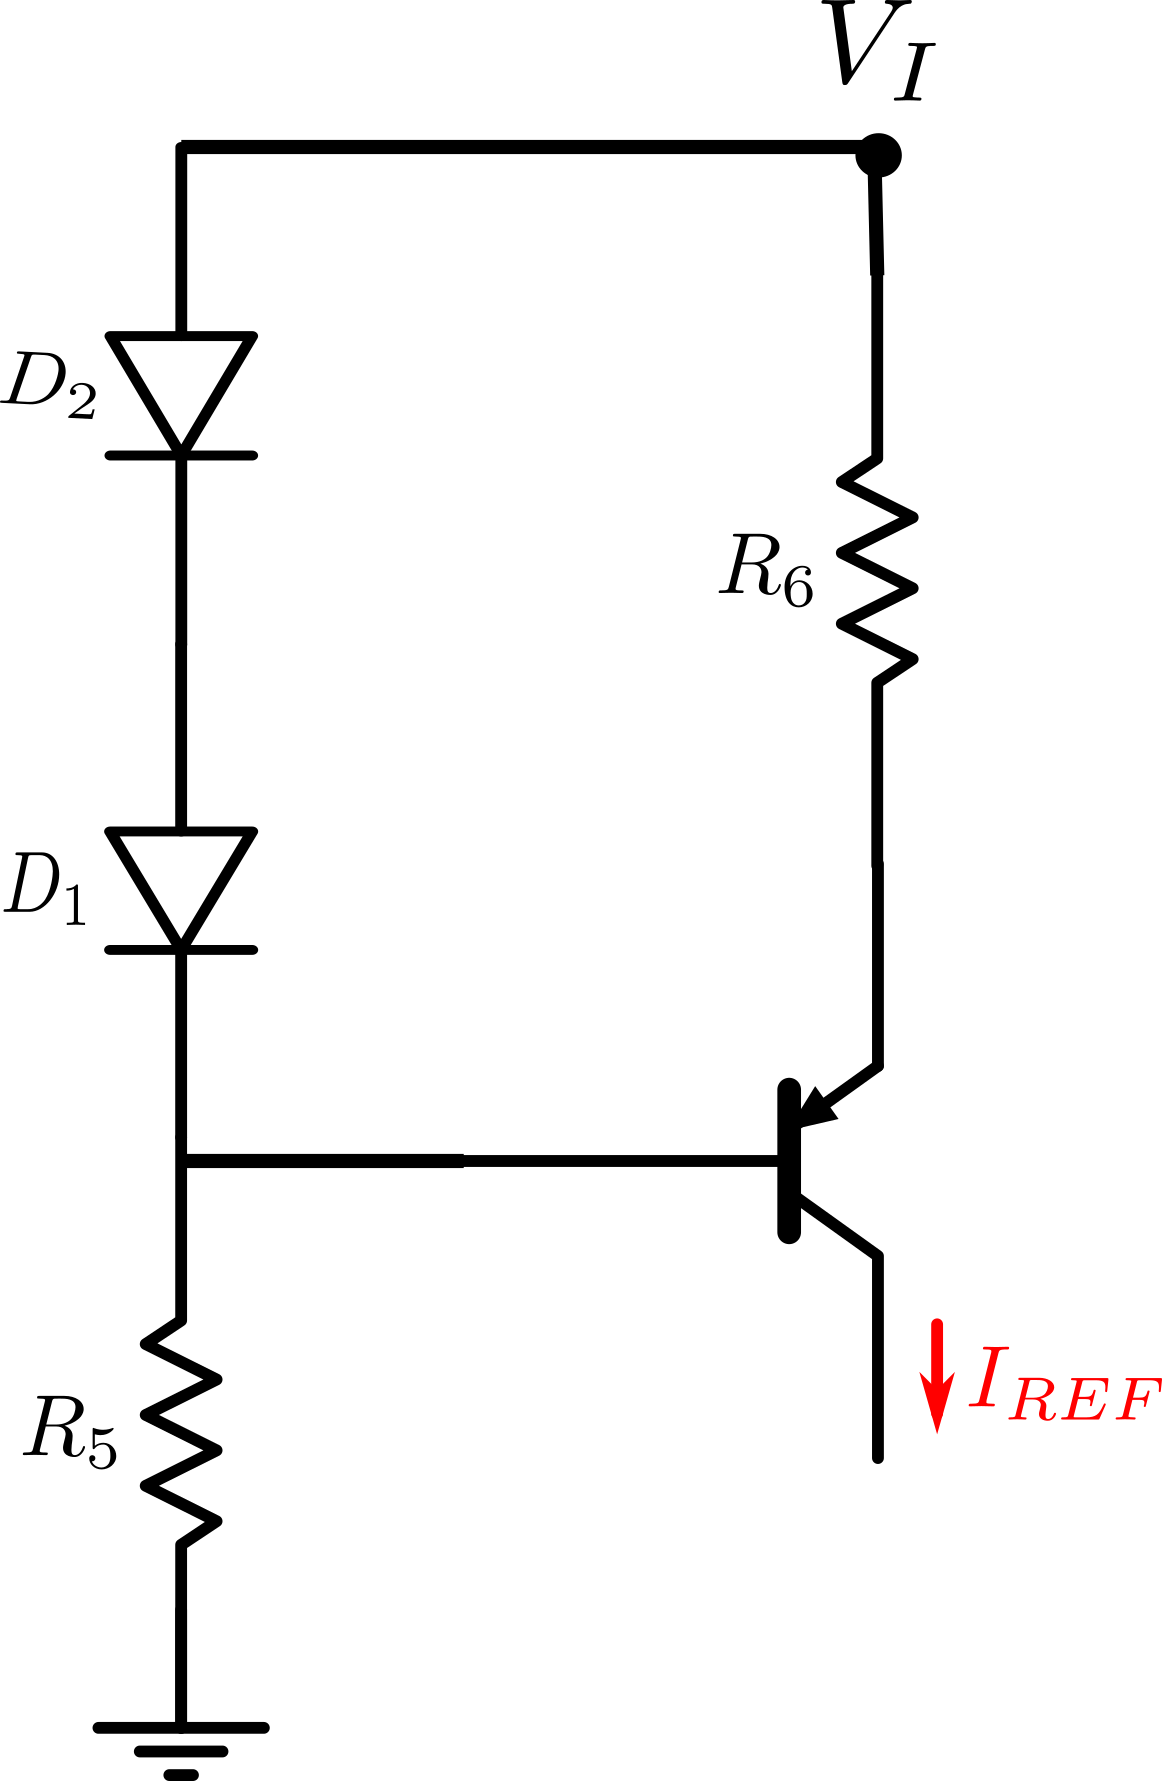
\includegraphics[scale=0.5]
	{circuitos/fuente.png}
	\caption{Fuente de corriente utilizada en el regulador de tensi\'on}
	\label{fig:fuente}
\end{figure}

Por lo tanto, como la corriente de salida es aproximadamente igual a la de $R_6$ (despreciando $I_{B_3}$), se obtiene:
\begin{equation}
	I_{REF} = \frac{0.7V}{R_6}
\end{equation}

Si sobredimensionamos la corriente m\'axima un 10\% (considerando las aproximaciones que se hicieron, posibles diferencias en las $V_D$ y $V_{BE}$ con los 0.7V te\'oricos, etc), se obtiene:
\[
	I_{REF} =
	 \frac{1.1 \cdot I_{O\, MAX}}
	 {\beta_{MIN\, 1} \cdot \beta_{MIN\, 2}}		
	 = \frac{1.1 \cdot 1.5\mathrm{A}}{100 \cdot 15}
	=1.1\text{mA}
\]

Por lo tanto, se eligieron los componentes:

\begin{itemize}
	\item $R_5$ = 10k$\Omega$, con lo cual los diodos se polarizan con una corriente de entre 0.96mA y 1.86mA (dado que la hoja del 1N4148 recomienda 1mA si se quiere 0.7V).
	\item $R_6$ = 642$\Omega$ (560 $\Omega$ en serie con $82\Omega$), con lo cual se tiene $I_{O\, MAX} \simeq 1.6355$A, que es lo m\'as cercano que se pudo llegar, con valores comerciales, a los 1.65A que se propuso.
	\item $T_3$ = BC557, un transistor PNP de uso general, que era el m\'as barato (la mitad que el siguiente m\'as barato) y con mayor disponibilidad del pa\~nol de la universidad, y con $I_C = 100$mA y $V_{CE}=45$V es m\'as que suficiente para este uso.
\end{itemize}


\end{document}

